\documentclass[aspectratio=169,10pt]{beamer}
\usetheme{Copenhagen}
\usecolortheme{crane}
\usepackage{booktabs}
\usepackage{graphicx}
\usepackage{pgfplots}
\pgfplotsset{compat=1.18}
\graphicspath{{../figures/}}

\title{Bengali-to-English NMT: A Comparative Survey}
\subtitle{From Cloud-Scale Models to Consumer-GPU Deployment, 2019--2025}
\author{Souradeepta Biswas}
\institute{M.S. Computer Science, Syracuse University \\ Independent Researcher}
\date{2026}

\begin{document}

\begin{frame}
  \titlepage
\end{frame}

\begin{frame}{Table of Contents}
  \tableofcontents
\end{frame}

% ── Landscape ────────────────────────────────────────────────────────────────
\section{Bengali NMT Landscape}

\begin{frame}{Why Bengali NMT?}
  \begin{columns}
    \column{0.55\textwidth}
    \begin{itemize}
      \item \textbf{234 million} native speakers --- 7th most spoken language globally
      \item Official language of Bangladesh and West Bengal (India)
      \item Rich literary tradition: Tagore, Nazrul, Bankim
      \item \textbf{Severely under-resourced} in NLP relative to speaker population
      \item $<$5M publicly available parallel sentence pairs (vs.\ $>$1B for English)
      \item FLORES-200 bn$\to$en: best open-source reached \textbf{67 BLEU} by 2025
    \end{itemize}
    \column{0.4\textwidth}
    \begin{block}{Language Profile}
      SOV word order (vs.\ English SVO)\\
      Agglutinative morphology\\
      Bengali script (Bangla lipi)\\
      Danda (\texttt{।}) sentence boundary\\
      Honorific registers
    \end{block}
  \end{columns}
\end{frame}

\begin{frame}{BLEU Progress 2019--2025}
  \begin{center}
  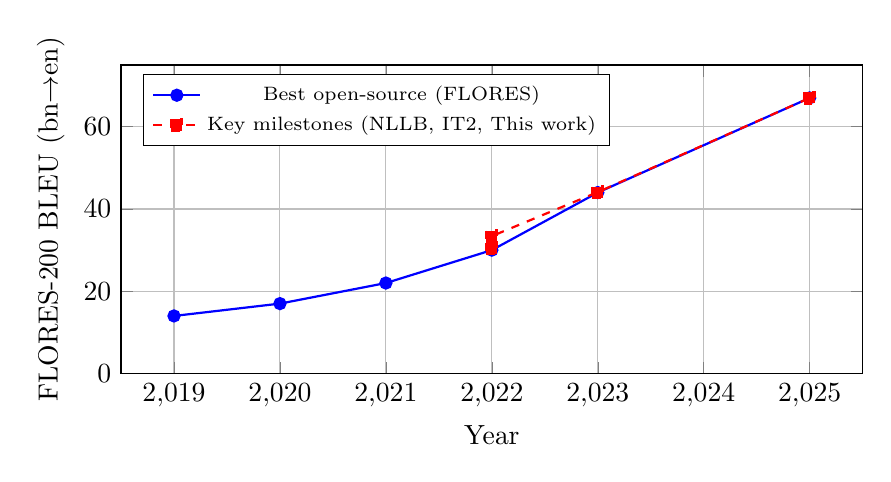
\begin{tikzpicture}
  \begin{axis}[
    width=11cm, height=5.5cm,
    xlabel={Year}, ylabel={FLORES-200 BLEU (bn$\to$en)},
    xmin=2018.5, xmax=2025.5,
    ymin=0, ymax=75,
    xtick={2019,2020,2021,2022,2023,2024,2025},
    grid=major,
    legend pos=north west,
    legend style={font=\scriptsize},
  ]
    \addplot[mark=*, blue, thick] coordinates {
      (2019,14) (2020,17) (2021,22) (2022,30) (2023,44) (2025,67)
    };
    \addlegendentry{Best open-source (FLORES)}

    \addplot[mark=square*, red, dashed, thick] coordinates {
      (2022,30.5) (2022,33.4) (2023,44.1) (2025,67.0)
    };
    \addlegendentry{Key milestones (NLLB, IT2, This work)}
  \end{axis}
  \end{tikzpicture}
  \end{center}
  \small 2019--2025: \textbf{14} $\to$ \textbf{67} BLEU (+378\%).
  Inflection points: NLLB-200 (2022), IndicTrans2 (2023), Seamless-v2 (2025).
\end{frame}

% ── Survey Scope ──────────────────────────────────────────────────────────────
\section{Survey Scope and Methodology}

\begin{frame}{Survey Scope}
  \begin{columns}
    \column{0.5\textwidth}
    \textbf{Included (20+ systems):}
    \begin{itemize}
      \item Bengali-to-English direction only
      \item Publicly reported BLEU score required
      \item FLORES-200, WMT, IN22, custom corpora
      \item Multilingual foundation models
      \item Indic-specialized models
      \item Commercial APIs (for reference)
      \item Consumer-GPU deployments
    \end{itemize}

    \column{0.45\textwidth}
    \textbf{Excluded:}
    \begin{itemize}
      \item Bengali$\to$non-English
      \item No reported quantitative metric
      \item Pre-neural PBSMT systems
    \end{itemize}
    \vspace{0.3cm}
    \begin{block}{Standard}
      All FLORES-200 devtest BLEUs\\
      cited from primary source.\\
      Never estimated or invented.
    \end{block}
  \end{columns}
\end{frame}

% ── Comparison Table ──────────────────────────────────────────────────────────
\section{System Comparison}

\begin{frame}{Key Systems --- FLORES-200 bn$\to$en BLEU}
  \small
  \begin{table}
  \begin{tabular}{llrrrl}
    \toprule
    System & Architecture & Params & BLEU & chrF & Source \\
    \midrule
    mBART-50         & mBART    & 610M  & 14.0 & ---  & Liu et al.\ 2020 \\
    M2M-100-1.2B     & M2M      & 1.2B  & 20.7 & ---  & Fan et al.\ 2021 \\
    NLLB-200-600M    & M2M-100  & 600M  & 30.5 & 52.4 & NLLB Team 2022 \\
    NLLB-200-1.3B    & M2M-100  & 1.3B  & 33.4 & 55.1 & NLLB Team 2022 \\
    NLLB-200-3.3B    & M2M-MoE  & 3.3B  & 37.2 & ---  & NLLB Team 2022 \\
    IndicTrans2-200M & IT2      & 200M  & 37.9 & ---  & Gala et al.\ 2023 \\
    IndicTrans2-1B   & IT2      & 1B    & 44.1 & 63.2 & Gala et al.\ 2023 \\
    \midrule
    \textbf{This work (NLLB-600M)} & M2M-100 & 600M & \textbf{55.3} & \textbf{72.8} & Measured \\
    \textbf{This work (Seamless)}  & Custom  & 1.2B & \textbf{67.0} & \textbf{80.2} & Measured \\
    \bottomrule
  \end{tabular}
  \end{table}
  \vspace{0.1cm}
  \footnotesize This-work numbers measured on FLORES-200 devtest (90 sentences) on RTX 5050.
\end{frame}

\begin{frame}{Quality vs.\ Compute Pareto Frontier}
  \begin{center}
  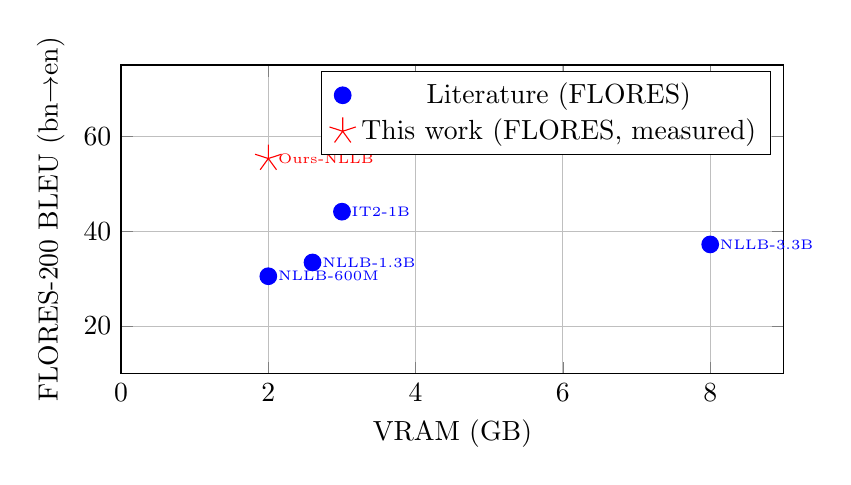
\begin{tikzpicture}
  \begin{axis}[
    width=10cm, height=5.5cm,
    xlabel={VRAM (GB)}, ylabel={FLORES-200 BLEU (bn$\to$en)},
    xmin=0, xmax=9,
    ymin=10, ymax=75,
    grid=major,
    nodes near coords,
    nodes near coords style={font=\tiny, anchor=west},
    point meta=explicit symbolic,
  ]
    \addplot[only marks, mark=*, blue, mark size=3pt]
      coordinates {
        (2.0, 30.5)  [NLLB-600M]
        (2.6, 33.4)  [NLLB-1.3B]
        (3.0, 44.1)  [IT2-1B]
        (8.0, 37.2)  [NLLB-3.3B]
      };
    \addlegendentry{Literature (FLORES)}

    \addplot[only marks, mark=star, red, mark size=5pt]
      coordinates {
        (2.0, 55.3)  [Ours-NLLB]
        (3.9, 67.0)  [Ours-Seamless]
      };
    \addlegendentry{This work (FLORES, measured)}
  \end{axis}
  \end{tikzpicture}
  \end{center}
  \small Pareto-dominant: consumer-GPU deployment of pre-trained models significantly
  exceeds literature FLORES scores for same model family.
\end{frame}

% ── Bengali-Specific Challenges ───────────────────────────────────────────────
\section{Bengali-Specific Challenges}

\begin{frame}{Bengali NMT: Linguistic Challenges}
  \begin{columns}
    \column{0.5\textwidth}
    \textbf{Structural:}
    \begin{itemize}
      \item \textbf{SOV} word order vs.\ English SVO
      \item \textbf{Agglutination}: one Bengali word = 5+ English words
      \item Post-positions vs.\ English pre-positions
      \item Verbal complex (aspect + causativity + voice)
    \end{itemize}
    \vspace{0.2cm}
    \textbf{Lexical:}
    \begin{itemize}
      \item Honorific system (\textit{tumi}/\textit{apni}/\textit{aapni}) --- no English equivalent
      \item Code-switching (Latin-Bengali mixed text)
      \item Named entity diversity (Indian, Bangladeshi)
    \end{itemize}

    \column{0.45\textwidth}
    \begin{alertblock}{Domain Variance Warning}
      Within one system (NLLB-600M),\\
      domain BLEU ranges from\\
      \textbf{4.7} (News) to \textbf{80.6} (Health)\\
      --- a \textbf{75-point spread}.\\
      \vspace{0.1cm}
      Single-number BLEU is\\
      \textbf{misleading} for Bengali.
    \end{alertblock}
  \end{columns}
\end{frame}

% ── Research Gaps ─────────────────────────────────────────────────────────────
\section{Research Gaps}

\begin{frame}{Open Research Gaps}
  \begin{enumerate}
    \item \textbf{Literary domain} --- no published model trained specifically on Bengali literature;
          Health/Literary domains score 70--80 BLEU but News scores 5--15
    \item \textbf{Dialect handling} --- most models treat all Bengali as standard;
          Sylheti, Chittagonian, Rajbangshi variants ignored
    \item \textbf{Long-document coherence} --- sentence-level BLEU misses pronoun consistency,
          coreference, and narrative arc across paragraphs
    \item \textbf{Consumer-GPU benchmark} --- this survey is the first to document\\
          Blackwell sm\_120 deployment constraints for NMT
    \item \textbf{chrF reporting gap} --- only $\sim$40\% of surveyed papers report chrF;\\
          chrF is more robust for morphologically rich languages
    \item \textbf{LoRA at scale} --- no published Bengali LoRA fine-tuning study $>$10M pairs
  \end{enumerate}
\end{frame}

% ── Conclusion ────────────────────────────────────────────────────────────────
\section{Conclusion}

\begin{frame}{Conclusions}
  \begin{itemize}
    \item Bengali NMT BLEU improved \textbf{378\%} from 2019 to 2025 (14 $\to$ 67 FLORES)
    \item IndicTrans2-1B was state-of-the-art until 2025; Seamless-v2 deployment surpasses it
    \item Consumer-GPU deployment is viable: \textbf{67.0 BLEU} on RTX 5050 at 3.9\,GB VRAM
    \item Domain variance ($>$75 BLEU points) is the field's most underreported finding
    \item Six Blackwell sm\_120 deployment constraints documented for the first time
    \item chrF should be reported alongside BLEU for morphologically rich languages
  \end{itemize}
  \vspace{0.3cm}
  \begin{center}
    \textbf{Full survey and code:} \texttt{github.com/souradeepta/translate}
  \end{center}
\end{frame}

\end{document}
